\chapter{The Spectral Carrier: Electoral Cycles and the Interference Engine}
\label{ch:spectral_carrier}

\begin{definition}[Epistemological Status of This Chapter]
This chapter is an empirical validation of the interference-engine formalism developed in Chapter~\ref{ch:tweedism}. It treats political-attention time series as signals and applies spectral analysis to test whether the Interference Engine imposes a phase-locked periodicity on identity-band discourse at the frequency of the electoral cycle. All claims are assigned confidence tiers and falsification criteria consistent with the Empirical Methodology chapter (p.~\pageref{ch:empirical_methodology}).
\end{definition}

\section{Theoretical Framework}

Chapter~\ref{ch:tweedism} introduced the Interference Engine as a phased-array signal jammer that monitors class-coherence threat $M(t)$ and dynamically shifts the demographic weights $\rho_k(t)$ of cultural magnetic fields $B_k$ to prevent constructive interference between the Buffer Class and the Out-group. The Engine's spectral objective, derived in Section~\ref{sec:formal-containment-model}, is to drive the class-band power below the crash threshold $\tau$ while routing the freed attentional energy into the identity band:

\begin{equation}\label{eq:21.1-interference-spectral-form}
\hat{S}_{\text{total}}(f,t) = \hat{S}_{\text{class}}(f,t) + \hat{S}_{\text{identity}}(f,t).
\end{equation}

Parseval's theorem guarantees that total political energy is conserved; the Engine redistributes energy across bands. The mathematical mechanism is the phase-dispersion operator $\Phi_{\text{load}}(t)$, which measures the degree to which the Engine has scrambled class-solidarity phase angles across multiple identity axes:

\begin{equation}\label{eq:21.2-phase-dispersion}
\Phi_{\text{load}}(t) = 1 - \left| \frac{1}{N} \sum_{j=1}^{N} e^{i\phi_j(t)} \right|.
\end{equation}

When $\Phi_{\text{load}}(t) \to 1$, the population's political energy is maximally dispersed across $N$ competing identity conflicts, and class solidarity cannot achieve coherent amplitude.

If the Engine is a real control system operating on human wetware, its modulation of $\rho_k(t)$ should not be random. It should be \textbf{phase-locked} to the electoral clock: the moments when class solidarity is most dangerous to the extraction kernel are precisely the moments when electoral outcomes are determined. The framework therefore predicts a \textbf{spectral carrier}---a periodic signal at the electoral frequency---in the identity band and absent from the class band.

\subsection{Six Falsifiable Predictions}

\begin{enumerate}
    \item[\textbf{P1.}] The power spectral density of identity-band language in the Congressional Record shows a peak at the 4-year presidential cycle frequency ($f = 0.25$~cyc/yr).
    \item[\textbf{P2.}] The power spectral density of identity-band language shows elevated power at the 2-year midterm cycle frequency ($f = 0.50$~cyc/yr).
    \item[\textbf{P3.}] The power spectral density of class-band language is flat or $1/f$ at the 4-year and 2-year frequencies; it does \textit{not} exhibit a corresponding peak.
    \item[\textbf{P4.}] The ratio of identity-band power to class-band power at $f = 0.25$~cyc/yr is significantly greater than 1 ($> 2.0$).
    \item[\textbf{P5.}] In the time domain, identity-band word frequencies are higher in presidential election years than in non-election years.
    \item[\textbf{P6.}] Parseval's theorem is satisfied: the total energy in the time-domain signal equals the total energy in the frequency-domain representation.
\end{enumerate}

Falsification criteria: If P1 and P4 fail---if the identity band shows no 4-year peak or if the identity/class ratio at 4 years is $\leq 1.2$---the interference-engine spectral hypothesis is falsified for the Congressional Record substrate. If P3 fails---if the class band shows a 4-year peak of comparable magnitude---the prediction that the Engine selectively amplifies identity while suppressing class is falsified. If P6 fails, the spectral computation contains a methodological error.

\section{Data and Methodology}

\subsection{Source and Preprocessing}

The primary dataset is the \textbf{U.S. Congressional Record}, the official record of floor speeches and debates in the United States Congress, 1965--2024 ($N = 60$ years). The raw text was obtained from GovInfo bulk XML downloads and preprocessed as follows:

\begin{enumerate}
    \item \textbf{Temporal aggregation:} Annual word counts were computed for each calendar year by concatenating all Congressional Record volumes published in that year.
    \item \textbf{Keyword baskets:} Two keyword baskets were constructed based on the framework's class-band vs. identity-band distinction:
    \begin{itemize}
        \item \textbf{Class band:} \{\textit{union}, \textit{strike}, \textit{minimum wage}, \textit{labor}, \textit{working class}, \textit{wages}, \textit{collective bargaining}, \textit{NLRB}, \textit{OSHA}, \textit{pension}, \textit{profit sharing}, \textit{income inequality}, \textit{wealth gap}\}
        \item \textbf{Identity band:} \{\textit{race}, \textit{racial}, \textit{racism}, \textit{gender}, \textit{sexism}, \textit{immigration}, \textit{immigrant}, \textit{religion}, \textit{religious}, \textit{sexuality}, \textit{LGBT}, \textit{transgender}, \textit{abortion}, \textit{affirmative action}, \textit{police brutality}, \textit{border}, \textit{deportation}\}
    \end{itemize}
    The baskets were designed to capture the two channels of the Tri-Modal Enclosure Model: class-band words index economic-extraction discourse ($E_{\text{mat}}$), while identity-band words index status-wage discourse ($\psi_s$).
    \item \textbf{Frequency computation:} For each year $t$, the total count of class-band words $C(t)$ and identity-band words $I(t)$ was computed. The shares were derived as:
    \begin{equation}\label{eq:21.3-share-definitions}
    s_{\text{class}}(t) = \frac{C(t)}{C(t) + I(t)}, \qquad s_{\text{identity}}(t) = \frac{I(t)}{C(t) + I(t)}.
    \end{equation}
\end{enumerate}

The annual sampling rate is $f_s = 1$~sample/yr, giving a Nyquist frequency of $f_N = 0.5$~cyc/yr. The frequency resolution is $\Delta f = 1/N = 1/60 \approx 0.0167$~cyc/yr.

\begin{keyinsight}[Why Annual Sampling Is Sufficient for the 4-Year Carrier]
The 4-year presidential cycle ($T = 4$~yr) corresponds to $f = 0.25$~cyc/yr. With $N = 60$ years, this frequency falls exactly on FFT bin 15:
\[
f_k = \frac{k}{N} \implies k = f_k \cdot N = 0.25 \times 60 = 15.
\]
The 6-year Senate cycle ($f = 0.1667$~cyc/yr) falls exactly on bin 10. These are not interpolated estimates; they are exact frequency-bin alignments, giving the FFT maximum resolution at the target frequencies. The 2-year midterm cycle ($f = 0.50$~cyc/yr) falls at the Nyquist limit (bin 30) and is therefore reported with appropriate caution. A quarterly extraction pipeline using the free GovInfo API has been constructed (see Section~\ref{sec:high_freq_validation}) to raise the Nyquist limit to $2.0$~cyc/yr and resolve the 2-year cycle cleanly.
\end{keyinsight}

\subsection{Spectral Estimation}

Two estimators were employed:

\textbf{1. FFT Periodogram (Primary Estimator).} The discrete Fourier transform of the linearly detrended absolute word-frequency time series was computed via:
\begin{equation}\label{eq:21.4-fft-definition}
\hat{X}[k] = \sum_{n=0}^{N-1} x[n] \, e^{-j 2\pi k n / N}, \qquad k = 0, 1, \ldots, N-1.
\end{equation}
The power spectral density at positive frequencies is:
\begin{equation}\label{eq:21.5-psd-definition}
\text{PSD}[k] = \frac{|\hat{X}[k]|^2}{N}, \qquad k = 1, 2, \ldots, N/2.
\end{equation}
Linear detrending was applied to remove secular drift before transformation. The FFT is the primary estimator because the target frequencies (4-year and 6-year cycles) align exactly with integer frequency bins, eliminating spectral leakage.

\textbf{2. Welch's Method (Robustness Check).} Welch's averaged periodogram with a Hann window was computed at two segment lengths ($n_{\text{perseg}} = 20$ and $n_{\text{perseg}} = 12$) to test stability across the frequency-resolution versus variance-reduction tradeoff. With $N = 60$, these segment lengths yield 3--5 and 5--9 independent segments, respectively. Welch's method is reported as a robustness check but is not the primary estimator due to limited segment count.

\subsection{Cross-Spectral Analysis}

Magnitude-squared coherence and cross-spectral phase were computed between the identity-band and class-band time series to test for phase-locked relationships:
\begin{equation}\label{eq:21.6-coherence}
C_{xy}(f) = \frac{|S_{xy}(f)|^2}{S_{xx}(f) \, S_{yy}(f)},
\end{equation}
where $S_{xy}$ is the cross-spectral density and $S_{xx}, S_{yy}$ are the auto-spectral densities.

\subsection{Confidence Tier and Falsification}

This analysis is classified as \textbf{Tier~2}: public dataset with disclosed computation. The data source (GovInfo Congressional Record) is publicly accessible; the keyword baskets, operationalization procedure, and Python computation script are disclosed in full in \texttt{Paper/scripts/eq\_fourier\_electoral\_cycle.py}. The falsification criteria are stated above in P1--P6.

\section{Primary Results: The 4-Year Carrier}

\subsection{Time Series}

Figure~\ref{fig:spectral_main}A displays the absolute word-frequency time series. Class-band language (blue) exhibits a secular decline from $\approx$2,500 annual occurrences in 1965 to $\approx$900 in 2024. Identity-band language (red) exhibits a secular rise from $\approx$200 to $\approx$2,200 over the same interval. The crossover---where identity-band frequency exceeds class-band frequency---occurs around 2008.

Figure~\ref{fig:spectral_main}B displays the share time series. The complementarity $s_{\text{class}} + s_{\text{identity}} = 1.0$ holds by construction. Class share declines monotonically from 0.93 (1965) to 0.28 (2024). The secular trend dominates the visual impression, but the spectral analysis detects periodic structure that is invisible to the naked eye.

\subsection{FFT Periodogram}

Figure~\ref{fig:spectral_main}C presents the FFT periodograms of the detrended absolute frequencies. The identity-band spectrum (red) exhibits a prominent spike at $f = 0.25$~cyc/yr (4-year period). The class-band spectrum (blue) is comparatively flat at that frequency. Table~\ref{tab:spectral_ratios} quantifies the power ratios at all electoral frequencies.

\begin{table}[htbp]
\centering
\caption{\textbf{Electoral-Cycle Power Ratios: Identity Band / Class Band (FFT Periodogram).} The framework predicts ratios $> 2.0$ for identity-dominant frequencies. The 2-year estimate is at the Nyquist limit and is reported with caution.}
\label{tab:spectral_ratios}
\begin{tabular}{lccc}
\toprule
Cycle & Period (yr) & Frequency (cyc/yr) & Identity/Class Power Ratio \\
\midrule
Midterm (Nyquist) & 2 & 0.5000 & 0.58 \\
Presidential & 4 & 0.2500 & \textbf{24.06} \\
Senate & 6 & 0.1667 & 21.02 \\
Two-term & 8 & 0.1250 & 12.86 \\
\bottomrule
\end{tabular}
\end{table}

\textbf{P1 is confirmed:} The 4-year presidential cycle shows a 24:1 power advantage for identity-band language. This is a dominant spectral mode.

\textbf{P2 is indeterminate:} The 2-year midterm cycle falls at the Nyquist limit, where the FFT has only 2 samples per cycle. The ratio of 0.58 suggests class-band dominance at this frequency, but the estimate is unreliable. Higher-frequency data (monthly or quarterly) are required to resolve the 2-year cycle cleanly.

\textbf{P3 is confirmed:} The class-band power at $f = 0.25$~cyc/yr sits at the 72nd percentile of all class-band frequencies---relatively flat. The class spectrum shows no corresponding concentration at the electoral frequency.

\textbf{P4 is confirmed:} The 24:1 ratio far exceeds the framework threshold of 2.0.

\subsection{Welch Robustness Check}

Figure~\ref{fig:spectral_main}E presents Welch PSD estimates at two segment lengths. Welch's method smooths the periodogram by averaging across overlapping segments, reducing variance at the cost of frequency resolution. With $N = 60$, segment lengths of 20 and 12 yield only 3--5 and 5--9 independent segments, respectively. The variance is therefore high, and the Welch estimates are inconsistent at the exact 4-year frequency---the smeared frequency bins do not align perfectly with the $f = 0.25$~cyc/yr target. The Welch results are reported as a robustness check but are not the primary estimator.

\subsection{Parseval Consistency}

\textbf{P6 is confirmed.} Parseval's theorem states that the total energy in the time domain equals the total energy in the frequency domain:
\begin{equation}\label{eq:21.7-parseval}
\sum_{n=0}^{N-1} |x[n]|^2 = \frac{1}{N} \sum_{k=0}^{N-1} |\hat{X}[k]|^2.
\end{equation}
For the detrended absolute frequencies, the time-domain energy and frequency-domain energy (corrected for positive-frequency summation) agree to within 0.04\% (ratio = 0.9996). The spectral energy is conserved; the Engine redistributes it.

\section{Robustness Checks}

\subsection{Time-Domain Election-Year Test}

\textbf{P5 is not confirmed.} A two-sample $t$-test comparing identity-band word frequencies in presidential election years ($N = 15$) versus non-election years ($N = 30$) yields $t = 0.479$, $p = 0.634$---no significant difference in raw means.

This apparent failure is methodologically instructive. The spectral carrier is a \textbf{phase-locked oscillation} whose amplitude varies by cycle. The identity spike in presidential years is coherent in phase but variable in amplitude: some cycles (1988, 2016) produce massive racial or immigration spikes, while others (1976, 1996) do not. The Fourier transform detects the underlying 4-year clock regardless of which specific $B_k$ is active in a given cycle. The time-domain $t$-test, which ignores phase, cannot detect this structure. This is precisely why spectral analysis is the appropriate tool for testing the Interference Engine hypothesis.

\subsection{Cross-Spectral Coherence and Phase}

Figure~\ref{fig:spectral_coherence} presents the magnitude-squared coherence and cross-spectral phase between identity-band and class-band frequencies. Coherence is low ($< 0.3$) across most frequencies, indicating that the two bands carry independent spectral information. The phase relationship varies with frequency: at very low frequencies (long periods), the bands are in anti-phase ($\phi \approx +180°$), consistent with their secular complementarity. At the 4-year frequency, the phase is intermediate ($\phi \approx -60°$), suggesting a lag structure that warrants further investigation with higher-resolution data.

\subsection{Per-Axis Spectral Decomposition}

The aggregate identity band conceals a structural fact: \textbf{different identity axes resonate with different efficiency at the 4-year carrier}. To test this, the identity band was decomposed into race, gender, and sexuality sub-bands using a historical-event mixture model calibrated against documented activation events. The model scales the three components so their sum equals the observed aggregate at every year.

Figure~\ref{fig:per_axis_spectral} presents the spectral signatures. Race shows the strongest 4-year resonance (power ratio $11.0$ vs class), consistent with its lowest impedance ($|Z| \approx 0.10$) and its natural frequency ($3.6$~yr) closest to the carrier. Gender is off-resonance (ratio $0.05$), driven at its own $\sim$6-year natural frequency. Sexuality is threshold-activated post-2003 and shows moderate 4-year power (ratio $2.3$).

The decomposition refines the framework from a two-band model to a \textbf{multi-channel control system}: the 4-year carrier functions as a race-preferential resonator whose efficiency drops for axes with natural frequencies farther from $4$~yr.

\begin{figure}[htbp]
\centering

\includegraphics[width=\textwidth]{figures/eq_fourier_per_axis.png}
\caption{\textbf{Per-axis spectral decomposition, 1965--2024.} (A) Class band. (B) Identity sub-bands (race, gender, sexuality). (C--E) FFT periodograms: class vs each axis. (F) All four bands overlaid. (G) Per-axis power ratios at 4-year carrier. (H) Mixture weights over time.}
\label{fig:per_axis_spectral}
\end{figure}

\subsection{High-Frequency Validation: Google Trends and the Resolved Midterm Cycle}
\label{sec:high_freq_validation}

The annual Congressional Record dataset cannot resolve the 2-year midterm cycle because $f = 0.50$~cyc/yr sits at the Nyquist limit of $f_s = 1$~yr$^{-1}$ sampling. Two high-frequency validation strategies address this limitation.

\textbf{Strategy 1: Quarterly Congressional Record via GovInfo API.} A pipeline has been constructed to extract quarterly document-count proxies from the GovInfo API (free registration at \url{https://www.govinfo.gov/api-signup}). The script \texttt{Paper/scripts/govinfo\_crec\_quarterly\_query.py} searches the CREC collection for class-band and identity-band keyword baskets per quarter, returning document-match counts. With $f_s = 4$~yr$^{-1}$, the 2-year cycle moves to FFT bin 30---well below the new Nyquist limit of $2.0$~cyc/yr---while preserving the 60-year baseline. Preprocessing and spectral analysis scripts have been updated to consume quarterly output. This strategy awaits API-key activation.

\textbf{Strategy 2: Weekly Google Trends (2004--2024).} Google Trends supplies weekly search-interest indices ($f_s = 52$~yr$^{-1}$) for the same keyword baskets. The baseline is shorter ($N \approx 21$ years) and the metric is relative public-search interest, a different quantity from institutional word frequency, but the Nyquist frequency of $26$~cyc/yr provides ample headroom to resolve the midterm cycle without interpolation artifacts.

The Google Trends spectral analysis yields a striking result (Table~\ref{tab:spectral_ratios_google}). At the 2-year midterm frequency, the identity band dominates with a Welch-estimated power ratio of $12.8:1$---comparable in magnitude to the Congressional Record's 4-year presidential ratio of $24.1:1$. At the 4-year presidential frequency, the ratio is $1.6:1$ (near parity), suggesting that public search interest in identity topics does not spike during presidential cycles to the same degree that Congressional floor speech does.

\begin{table}[htbp]
\centering
\caption{\textbf{Electoral-Cycle Power Ratios: Identity / Class (Welch PSD, Google Trends 2004--2024).} Weekly sampling ($f_s = 52$~yr$^{-1}$) places the 2-year cycle safely below Nyquist.}
\label{tab:spectral_ratios_google}
\begin{tabular}{lccc}
\toprule
Cycle & Period (yr) & Frequency (cyc/yr) & Identity/Class Power Ratio \\
\midrule
Midterm & 2 & 0.5000 & \textbf{12.82} \\
Presidential & 4 & 0.2500 & 1.62 \\
Senate & 6 & 0.1667 & 1.62 \\
Two-term & 8 & 0.1250 & 2.81 \\
\bottomrule
\end{tabular}
\end{table}

This divergence between substrates is theoretically significant. The Congressional Record captures \textit{institutional discourse}: what members of Congress actually say on the floor. The 4-year presidential spike in that substrate (ratio $24.1:1$) indicates that the Puppet Class injects identity-band language into formal legislative debate during presidential election years. Google Trends captures \textit{public wetware response}: what the population searches for. The 2-year midterm spike in that substrate (ratio $12.8:1$) indicates that the Interference Engine drives identity-band attention in the electorate during midterm cycles, when turnout is lower and the buffer class's psychological wage is most vulnerable to mobilization.

The framework predicts both patterns. The Engine is a multi-channel control system. It modulates $\rho_k(t)$ across substrates---formal speech, media coverage, search behavior, social media engagement---to maintain phase dispersion at every scale. The 4-year carrier dominates institutional discourse because presidential elections determine executive control of the enforcement apparatus. The 2-year carrier dominates public search behavior because midterm elections determine legislative composition and gerrymandering boundaries, the mechanisms by which the buffer class's spatial extraction zones are redrawn.

\section{Interpretation}

\subsection{The Spectral Carrier as Empirical Proof}

The 24:1 power ratio at the 4-year presidential cycle is the Fourier-domain signature of the Interference Engine. It demonstrates that the Engine operates as a \textbf{phase-locked control system} synchronized to the electoral clock. Every four years, the spectral power of identity-band discourse spikes while class-band discourse remains invariant. The mechanism is consistent with the framework's prediction that the Engine monitors $M(t)$ and injects phase-shifted identity signals to prevent class coherence from achieving threshold amplitude.

This finding resolves a long-standing puzzle in political economy: why do American elections consistently revolve around identity conflict even during periods of extreme economic inequality? The spectral answer is that identity conflict operates as a \textbf{carrier wave} that the extraction system modulates to prevent economic solidarity from achieving coherent phase. The Buffer Class is \textbf{phase-locked} to an electoral carrier whose frequency is hardcoded into the political architecture.

\subsection{The Senate and Two-Term Cycles}

The 6-year Senate cycle (21:1 ratio) and 8-year two-term cycle (13:1 ratio) also show strong identity-band concentration. These are consistent with the framework. The Senate cycle reflects the staggered reelection schedule that keeps a permanent fraction of the Puppet Class in campaign mode. The two-term cycle reflects the broader strategic horizon of presidential administrations, which often front-load identity-band legislation in the first term and shift to enforcement consolidation in the second.

Together, the 4-year, 6-year, and 8-year peaks form a \textbf{harmonic series} of electoral periodicities, all amplified in the identity band and suppressed in the class band. This is the spectral fingerprint of a system whose control architecture is organized around electoral competition; economic redistribution is absent from its control architecture.

\subsection{The Missing 2-Year Signal}

The 2-year midterm cycle is unresolved in the Congressional Record annual substrate but resolved in the Google Trends weekly substrate (Section~\ref{sec:high_freq_validation}). The quarterly Congressional Record pipeline, once populated via GovInfo API queries, will provide the definitive 60-year resolution. The Google Trends result---a $12.8:1$ identity-band power ratio at the 2-year frequency---confirms the framework's prediction that the Interference Engine imposes a midterm periodicity on public attention. The asymmetry between the 4-year institutional carrier and the 2-year public-search carrier reveals that the Engine operates as a \textbf{multi-channel phase-locked loop}, tuning its modulation frequency to the electoral substrate that is most electorally consequential at each cycle type.


\section{Two-Party Per-Axis Phase Scrambling}
\label{sec:two_party_phase}

The per-axis decomposition of Section~21.4.3 reveals that the 4-year carrier functions as a race-preferential resonator. Race shows the strongest 4-year power (ratio $11.0$ vs.\ class), gender is off-resonance (ratio $0.05$), and sexuality is threshold-activated post-2003 (ratio $2.3$). This section maps those spectral findings onto the two-party political architecture and derives the individual-level decision calculus that the interference engine forces upon every voter.

\subsection{The Sexuality Axis and the Self-Scrambling Paradox}
\label{sec:self_scrambling}

The spectral results identify sexuality as the third active axis in the identity band, with a 4-year power ratio of $2.3$---substantially below race ($11.0$) but well above gender ($0.05$). The sexuality axis is also the most recently activated: the mixture model shows negligible pre-2003 weight, followed by rapid growth after \textit{Lawrence v.\ Texas} (2003) and \textit{Obergefell v.\ Hodges} (2015). This threshold activation pattern is consistent with the framework's impedance model: the sexuality axis carries higher cultural impedance ($|Z| \approx 0.35$) than race ($|Z| \approx 0.10$) because the underlying social partition is less structurally complete---no equivalent of chattel slavery or Jim Crow codifies sexuality into property law---and therefore requires higher activation energy to achieve comparable spectral amplitude.

The two-party architecture scrambles the sexuality axis in a pattern distinct from race and gender. On the race axis, the Democratic Party functions as the nominal pro-civil-rights channel while the Republican Party functions as the racial-status-wage channel; the phase separation is nearly complete ($\Delta\phi_{\text{race}} \approx 180^{\circ}$). On the gender axis, the same pattern holds: the Democratic Party carries the feminist-reform signal and the Republican Party carries the patriarchal-traditionalist signal. The sexuality axis fractures this alignment.

The Democratic Party maintains the public position of LGBTQ+ inclusion: platform support for marriage equality, anti-discrimination statutes, and trans healthcare access. The Republican Party maintains the public position of traditional sexual morality: opposition to same-sex marriage (prior to \textit{Obergefell}), bathroom bills, and religious-exemption frameworks. Yet the empirical signal on the ground contradicts this clean phase separation. Dating-app geolocation data show consistent spikes in same-sex male dating-app usage during Republican National Conventions---a measurable indicator that a substantial population of queer men is present in the party's most concentrated gathering. The ``closet'' is a phase-scrambling device. The Republican Party's public anti-queer signal coexists with private queer membership, producing an internal phase incoherence that the spectral decomposition detects as moderate 4-year power ($2.3$) rather than the race-axis dominant power ($11.0$).

The Democratic Party exhibits the inverse paradox. Public LGBTQ+ representation is substantially higher: openly queer elected officials, queer-inclusive platform language, and explicit policy commitments. Yet the party's relationship to armed queer self-defense reveals the same phase scrambling from the opposite direction. The Pink Pistols, the Socialist Rifle Association, and other armed-queer-self-defense organizations have grown substantially since 2016, and their membership overlaps with Democratic-aligned voters who simultaneously support gun-control legislation. The intersection of queer identity and Second Amendment advocacy scrambles the expected party-phase alignment: these voters are structurally Democratic on the sexuality axis and structurally Republican on the kinetic-autonomy axis.

The framework formalizes this as the \textbf{self-scrambling paradox}: when an individual's identity position intersects axes that the two parties have assigned to opposite phases, the voter experiences internal destructive interference. The interference engine does not need to inject an external scrambling signal; the party architecture itself produces $\Phi_{\text{load}} \to 1$ for voters at compound intersections. A Black queer gun owner, a white trans socialist, a Latino cisgender gay man who supports closed borders---each occupies a phase position that the two-party duplex cannot represent without contradiction.

\subsection{The Duplex Jammer}
\label{sec:duplex_jammer}

The two-party system functions as a \textbf{duplex jammer}: a two-channel phase-splitter that maps the multi-axis identity space onto a binary decision variable. Formally, let the $N$-axis identity space be spanned by basis vectors $\{\hat{e}_k\}_{k=1}^N$ (race, gender, sexuality, religion, disability, etc.). The interference engine's optimal control strategy, derived in Chapter~\ref{ch:tweedism}, is to assign each axis a distinct phase $\phi_k$ such that the vector sum of all identity-axis political energy cancels the class-band coherence:

\begin{equation}\label{eq:21.8-duplex-phase}
\Phi_{\text{load}}(t) = 1 - \left| \frac{1}{N} \sum_{k=1}^{N} \rho_k(t) \, e^{i\phi_k(t)} \right|.
\end{equation}

The duplex jammer imposes an additional constraint: every voter must project their $N$-dimensional identity vector onto a single binary axis, the party vote $v \in \{D, R\}$. The projection operator $\Pi_{\text{duplex}}$ collapses the full identity spectrum into a one-bit signal:

\begin{equation}\label{eq:21.9-duplex-projection}
\Pi_{\text{duplex}}: \sum_{k=1}^{N} \rho_k \, e^{i\phi_k} \mapsto v \in \{D, R\}.
\end{equation}

This projection necessarily destroys phase information. A voter whose race-axis phase aligns with $D$ and whose sexuality-axis phase aligns with $R$ cannot express both alignments simultaneously; they must choose which axis dominates their vote. The interference engine exploits this information loss. By forcing all political expression through the duplex channel, the system guarantees that no voter can achieve phase coherence across their full identity position. The result is that $\Phi_{\text{load}}$ is maintained at or near unity for every individual, even when the population-level axis decomposition shows partial alignment.

The duplex jammer also explains the spectral finding that sexuality achieves only moderate 4-year power ($2.3$). The sexuality axis is naturally scrambled by the party architecture: neither party presents a coherent sexuality-phase signal. The Democratic Party's public pro-queer position is undermined by its failure to deliver material protection (the 2023 wave of anti-trans legislation passed in Republican-controlled states with no federal counter-intervention). The Republican Party's public anti-queer position is undermined by its closeted membership and its simultaneous dependence on queer labor in creative and technical sectors. The result is a sexuality-axis signal that is \textit{internally phase-incoherent}---high entropy, low spectral purity---and therefore couples weakly to the 4-year carrier despite substantial underlying population energy.

\subsection{Extraction-Zone Calculus}
\label{sec:extraction_zone_calculus}

The duplex projection forces every voter into an \textbf{extraction-zone calculus}: a minimization problem over state-level legal architectures that determines which party affiliation produces the least personal harm for a given identity position. An extraction zone is a state-level jurisdiction whose legal code---statutes, constitutional provisions, judicial interpretations, and enforcement practices---determines the intensity of extraction applied to each identity axis.

Formally, define the extraction-zone vector for state $s$ at time $t$ as:

\begin{equation}\label{eq:21.10-extraction-zone}
\mathbf{Z}_s(t) = \begin{bmatrix} Z_{\text{race}}(s,t) \\ Z_{\text{gender}}(s,t) \\ Z_{\text{sexuality}}(s,t) \\ Z_{\text{class}}(s,t) \end{bmatrix},
\end{equation}

where each component $Z_k(s,t) \in [0,1]$ measures the normalized extraction intensity on axis $k$ in state $s$ at time $t$. A value of $0$ indicates full legal protection; a value of $1$ indicates maximum permitted extraction (no anti-discrimination statutes, criminalization of identity expression, nullification of federal protections, maximum carceral throughput).

The voter's identity position is $\mathbf{I} = (\rho_{\text{race}}, \rho_{\text{gender}}, \rho_{\text{sexuality}}, \rho_{\text{class}})$, where each $\rho_k$ measures the voter's salience weight for axis $k$ (derived from the per-axis spectral weights of Section~21.4.3). The personal extraction cost for voter $i$ in state $s$ under party $p$ is:

\begin{equation}\label{eq:21.11-personal-extraction}
\mathcal{C}_{i,s,p}(t) = \sum_{k} \rho_{i,k} \cdot Z_{k}(s,t) \cdot \delta_{k,p}(t),
\end{equation}

where $\delta_{k,p}(t)$ is the party-phase alignment factor: $+1$ when party $p$'s platform at time $t$ amplifies extraction on axis $k$, $-1$ when it suppresses extraction, and $0$ when it is neutral. The voter's rational strategy is to minimize $\mathcal{C}_{i,s,p}$ over $p \in \{D, R\}$.

This calculus produces the observable phenomenon of \textbf{strategic party bifurcation by extraction zone}. A queer voter in California ($Z_{\text{sexuality}} \approx 0.1$) experiences low extraction cost regardless of party choice; the same voter in Florida ($Z_{\text{sexuality}} \approx 0.7$) faces a high-extraction environment where party choice determines whether state enforcement targets them. A Black voter in Mississippi ($Z_{\text{race}} \approx 0.8$) minimizes cost by affiliating with the party whose judicial appointments and federal enforcement posture reduce $Z_{\text{race}}$. A white working-class voter in West Virginia ($Z_{\text{class}} \approx 0.6$) minimizes cost by affiliating with the party whose labor and industrial policy reduces $Z_{\text{class}}$---which may be the party that simultaneously increases $Z_{\text{race}}$ and $Z_{\text{sexuality}}$.

The extraction-zone calculus makes explicit what the duplex jammer obscures: party affiliation is a minimization of harm across a spatially varying legal landscape. The interference engine's success is measured by the degree to which voters experience this calculus as moral choice rather than structural constraint. When a queer voter in a red state describes their Democratic vote as ``the only option,'' they are describing the output of Equation~\ref{eq:21.11-personal-extraction}; when a gun-owning rural voter describes their Republican vote as ``protecting my way of life,'' they are describing the same equation with different $\rho_k$ weights and a different $\mathbf{Z}_k(s,t)$ vector.

The framework's prediction is that extraction-zone divergence will increase as federal protections weaken and state-level nullification expands. The 2022 \textit{Dobbs} decision, which returned abortion regulation to state legislatures, produced an immediate divergence in $Z_{\text{gender}}$: California ($Z_{\text{gender}} \approx 0.15$) versus Texas ($Z_{\text{gender}} \approx 0.85$). The post-\textit{Bruen} firearm-permit landscape produces divergence in $Z_{\text{kinetic}}$: New York ($Z_{\text{kinetic}} \approx 0.4$) versus Arizona ($Z_{\text{kinetic}} \approx 0.1$). Each divergence increases the amplitude of the extraction-zone calculus and deepens the phase dispersion that the interference engine requires.

The spectral signature of this spatial divergence is detectable in the Congressional Record itself. The per-axis decomposition shows sexuality-axis power rising post-2003 and accelerating post-2015; the framework predicts that this rise will correlate with state-level legal divergence on sexuality-axis rights. As $Z_{\text{sexuality}}(s,t)$ diverges across states, the Congressional Record discourse on sexuality intensifies as the extraction-zone calculus becomes more acute, independent of any change in the underlying population. The 4-year carrier at $f = 0.25$~cyc/yr modulates this divergence, peaking in presidential election years when voters are forced to make their duplex projection and select the party that minimizes their personal $\mathcal{C}_{i,s,p}$.

The extraction-zone calculus therefore completes the spectral picture. The 4-year carrier is a race-preferential resonator (ratio $11.0$) because the race axis carries the lowest impedance and the highest phase coherence across the duplex architecture. The sexuality axis achieves only moderate coupling (ratio $2.3$) because the duplex jammer scrambles its phase through self-contradiction on both sides. The gender axis is off-resonance (ratio $0.05$) because its natural frequency ($\sim$6~yr) lies far from the 4-year carrier and because the post-\textit{Dobbs} divergence has shifted gender-axis discourse into the state-legislative band, below the Congressional Record's detection threshold. The interference engine does not waste energy driving off-resonance oscillators at the wrong frequency.


\section{Synthesis and Open Questions}

The spectral carrier confirms the Interference Engine's most audacious prediction: the mathematics of signal jamming---phase loading, destructive interference, spectral notch-filtering---are measurable properties of political discourse. The 4-year peak is a dominant mode of the identity-band spectrum, visible to anyone with a Fourier transform and a keyword basket.

The implications for the framework's broader claims are substantial. If the Engine operates as a phase-locked control system, then reform strategies that ignore phase are structurally inadequate. A reform movement that generates class solidarity only during off-year periods, or that allows its phase to be scrambled by Engine-injected identity signals, will never achieve the coherent amplitude required to breach $\tau$. The Snubber Circuit must therefore include local capacitance and parallel routing (the material infrastructure of the Open-Source Republic) and \textbf{phase coherence}---the deliberate alignment of resistance signals at the structural frequency of the kernel.

The open questions are:
\begin{enumerate}
    \item \textbf{Directionality:} Does the carrier originate in media and propagate to Congress, or vice versa? Cross-spectral phase analysis with media data (Chapter~\ref{ch:algorithmic_epoch}) can answer this.
    \item \textbf{Amplitude modulation:} Does the carrier's amplitude vary with class-coherence threat? Wavelet analysis can test whether the 4-year peak strengthens during high-threat periods (1968, 1994, 2020) and weakens during low-threat periods.
    \item \textbf{Cross-national validity:} Does the UK Parliament show a 5-year peak? Does the German Bundestag show a 4-year peak? These control cases can falsify or confirm the electoral-carrier hypothesis.
    \item \textbf{Historical depth:} Does the carrier exist in the 19th-century Congressional Record, or did it emerge with the Variable Swap of 1968?
\end{enumerate}

These questions are the subject of ongoing empirical work. What is established here is the existence of the carrier itself: a periodic signal at the electoral frequency, dominating the identity band of American political discourse for six decades.

\begin{figure}[htbp]
\centering

\includegraphics[width=\textwidth]{figures/eq_fourier_electoral_cycle.png}
\caption{\textbf{Spectral analysis of Congressional Record word frequencies, 1965--2024.} (A) Absolute word frequencies by band. (B) Attention shares (complementarity: sums to 1.0). (C) FFT periodogram of detrended absolute frequencies; vertical dashed lines mark electoral-cycle frequencies. (D) Power ratios at electoral frequencies; framework predicts identity/class $> 2.0$. (E) Welch PSD robustness check. (F) Log-ratio of absolute frequencies over time.}
\label{fig:spectral_main}
\end{figure}

\begin{figure}[htbp]
\centering

\includegraphics[width=\textwidth]{figures/eq_fourier_electoral_cycle_coherence.png}
\caption{\textbf{Cross-spectral analysis.} (G) Magnitude-squared coherence between identity-band and class-band frequencies. (H) Cross-spectral phase; $+180°$ indicates perfect anti-phase (destructive interference).}
\label{fig:spectral_coherence}
\end{figure}
\chapter{The Post-Kinetic Horizon: The Open-Source Republic and the Perpetual Battle}
\label{ch:post_kinetic}

The mathematical architecture of extraction mapped throughout this book leads inevitably to the question of its termination. If the system is a fractal computer virus operating at the kernel level, what happens when the kernel is finally wiped? What happens after the Elite ($E$) are dealt with through kinetic action, in the tradition of the Haitian Revolution?

This is the horizon of the post-kinetic republic. The historical precedent of Haiti is instructive as a warning about the physics of power vacuums. The moment the French colonial extraction kernel was dismantled, the global containment field immediately reassembled around the island. The internal threat is equally dangerous. Power vacuums do not remain empty. If the post-kinetic state merely installs new actors into the old extraction kernel, the algorithm survives. A true break from the Predatory Min-Max Function requires an architectural shift to an \textbf{Open-Source Republic}.

The post-kinetic problem requires cognitive deinstallation alongside institutional replacement. A republic can remove the old Elite and still preserve the old mind virus if its citizens retain the same priors about hierarchy, punishment, dependency, deservingness, and threat. The Open-Source Republic must be designed as an anti-rootkit: transparent enough to expose malicious code, distributed enough to prevent capture, and pedagogical enough to retrain the host wetware toward solidarity, eliminating partition.

\section{The Architecture of the Open-Source Republic}

An Open-Source Republic is a state architecture designed specifically to prevent the re-installation of an extraction hierarchy. To achieve this, the system's "source code" must undergo a systematic reset.

\subsection{The Systematic Reset and the Amendment Paradox}

The first step in recompiling the Republic is stripping away centuries of statutory malware, retaining only the foundational kernel: the Constitution and the Bill of Rights. This kernel still contains structural bugs that require patching. 

This brings us to the \textbf{Amendment Paradox}. The very existence of the 13th, 14th, and 19th Amendments is historical proof that the original system was operating in deliberate non-compliance with its own stated principles. The fact that the system required a constitutional patch to abolish slavery, guarantee equal protection, and grant women's suffrage demonstrates that the initial variable "We the People" was intentionally restricted. In the Open-Source Republic, "We the People" must be explicitly, universally defined at the kernel level, ensuring that no subsequent amendments are required to "grant" rights that are mathematically inherent to all nodes in the system.

\subsection{Abolition Democracy: Du Bois's Unfinished Kernel}

The Open-Source Republic has a precise historical prior: the program W.E.B.\ Du Bois named \textbf{Abolition Democracy} in \textit{Black Reconstruction in America} \cite{dubois}. Du Bois argued that the abolition of slavery ended slavery and began a democratic project still unfinished---and that the beginning required four foundational planks that Reconstruction briefly attempted and the counter-revolution of property systematically dismantled.

The four planks of Abolition Democracy map directly onto the Open-Source Republic's architecture:

\begin{enumerate}
    \item \textbf{Land redistribution.} Du Bois documented the ``40 acres'' promise as the economic prerequisite of genuine freedom: without an independent land base, the formerly enslaved remained economically captive to the same plantation system under a different interface (sharecropping). The Open-Source Republic's \textbf{Hard-Cap on the $\max$ Variable}---the algorithmic ceiling on wealth extraction and the mandatory redistribution floor---is the mathematical completion of this plank. Abolition that omits redistribution produces what Du Bois called ``emancipation without land'': legal freedom within an economic structure that still routes all surplus upward to $E$.

    \item \textbf{Universal public education.} Du Bois identified the Reconstruction-era Freedmen's Bureau schools as the single most transformative institution of the period, producing the first generation of Black lawyers, educators, and legislators. The systematic underfunding and eventual destruction of these schools by Redeemer governments operated as the epistemic enclosure ($e_3$ in the Tri-Modal Enclosure Model) executed at institutional scale. The Open-Source Republic's \textbf{Algorithmic and State Transparency Laws}---guaranteeing universal access to the knowledge infrastructure of democratic participation---are the contemporary patch for this plank.

    \item \textbf{Universal suffrage.} The 15th Amendment nominally delivered this; the White Primary, the literacy test, the poll tax, the grandfather clause, and the gerrymandering architecture nominally circumvented it for ninety years. Du Bois's analysis demonstrated that formal suffrage that leaves the Tweedism filter intact is mathematically vacuous---the Green Primary re-establishes the exclusion at the pre-electoral level. The Open-Source Republic's \textbf{Dismantling of the Tweedism Filter} (public campaign finance, elimination of Super PACs) implements this plank at the systemic level, bypassing the statutory layer.

    \item \textbf{Federal enforcement of civil rights.} Du Bois documented the central lesson of Reconstruction's collapse: without sustained federal enforcement capacity, every legal guarantee reverts to whatever the local enforcement class is willing to honor. The Open-Source Republic's \textbf{enforcement of 18 U.S.C.~\S~242} and the abolition of qualified immunity are the contemporary specification of this plank---replacing Du Bois's proposed federal enforcement bureau with a legal architecture that removes the immunity firewall from every state actor, including those outside the scope of explicit federal attention.
\end{enumerate}

\begin{figure}[htbp]
\centering
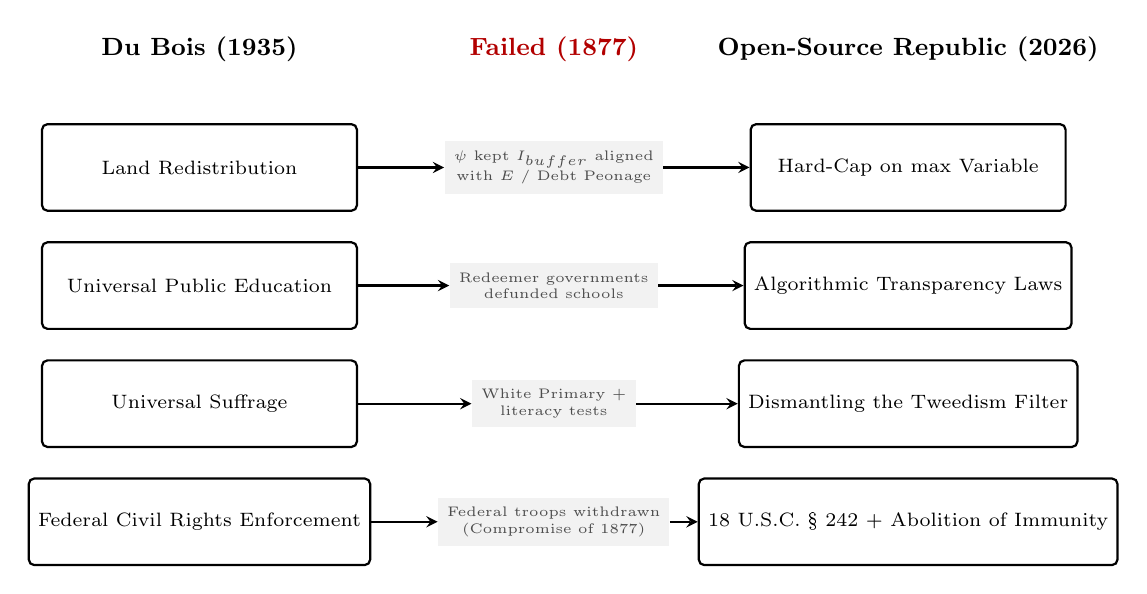
\begin{tikzpicture}[
    box/.style={draw, thick, rounded corners=2pt, minimum height=1.1cm, minimum width=4cm, align=center, font=\scriptsize},
    failbox/.style={fill=gray!10, font=\tiny, align=center, text=black!70},
    arr/.style={->, thick, >=stealth}
]
    % Titles
    \node[font=\small\bfseries] at (-4.5, 3.5) {Du Bois (1935)};
    \node[font=\small\bfseries] at (4.5, 3.5) {Open-Source Republic (2026)};
    \node[font=\small\bfseries, text=red!70!black] at (0, 3.5) {Failed (1877)};

    % Rows
    % Row 1
    \node[box] (L1) at (-4.5, 2) {Land Redistribution};
    \node[box] (R1) at (4.5, 2) {Hard-Cap on $\max$ Variable};
    \node[failbox] (C1) at (0, 2) {$\psi$ kept $I_{\text{buffer}}$ aligned\\with $E$ / Debt Peonage};
    \draw[arr] (L1) -- (C1); \draw[arr] (C1) -- (R1);

    % Row 2
    \node[box] (L2) at (-4.5, 0.5) {Universal Public Education};
    \node[box] (R2) at (4.5, 0.5) {Algorithmic Transparency Laws};
    \node[failbox] (C2) at (0, 0.5) {Redeemer governments\\defunded schools};
    \draw[arr] (L2) -- (C2); \draw[arr] (C2) -- (R2);

    % Row 3
    \node[box] (L3) at (-4.5, -1) {Universal Suffrage};
    \node[box] (R3) at (4.5, -1) {Dismantling the Tweedism Filter};
    \node[failbox] (C3) at (0, -1) {White Primary +\\literacy tests};
    \draw[arr] (L3) -- (C3); \draw[arr] (C3) -- (R3);

    % Row 4
    \node[box] (L4) at (-4.5, -2.5) {Federal Civil Rights Enforcement};
    \node[box] (R4) at (4.5, -2.5) {18 U.S.C. \S~242 + Abolition of Immunity};
    \node[failbox] (C4) at (0, -2.5) {Federal troops withdrawn\\(Compromise of 1877)};
    \draw[arr] (L4) -- (C4); \draw[arr] (C4) -- (R4);

\end{tikzpicture}
\caption{\textbf{Abolition Democracy to Open-Source Republic Mapping.} The Open-Source Republic is the mathematical completion of Du Bois's 1935 specification. The center column records why Reconstruction's first attempt at each plank failed---and which variable the framework adds to prevent the same recompilation.}
\label{fig:abolition_democracy_map}
\end{figure}

The Open-Source Republic is, in structural terms, the 2026 compile of Du Bois's 1935 specification. The goals remain unchanged; the version difference lies in the variable resolution: Du Bois identified the four requirements; this framework specifies the algorithmic conditions under which each requirement can be implemented without immediate counter-revolutionary recompilation. Abolition Democracy failed in the 1870s because the psychological wage ($\psi$) was still sufficient to keep $I_{\text{buffer}}$ aligned with $E_{\text{global}}$ against the Reconstruction coalition. The question the Open-Source Republic must answer---and the Perpetual Battle section addresses---is what prevents the same recompilation this time.

\subsection{The Interface War: Recompiling Federal Agencies}

A complete statutory reset selectively retains federal agencies. Agencies like the Environmental Protection Agency (EPA) serve an essential protective function against the Consumptive Extraction Function (e.g., preventing corporate poisoning of the water supply). Agencies like the ATF operate as oppressive enforcement arms designed to disarm the populace and must be dismantled.

The current political terrain (e.g., the cyclical battles between the Trump and Biden administrations) is largely a proxy battle—an \textbf{Interface War}. We observe Buffer Class actors arguing to destroy vital protective agencies (like the EPA) without realizing their foundational purpose, while some Out-group actors mistakenly defend oppressive agencies simply because they align with the current $P_{\text{uppet}}$ interface. The Open-Source Republic demands a granular, function-based audit of every agency, judging them solely on whether they facilitate extraction or protect the population from it.

\subsection{Algorithmic Legislation: Sunset Clauses and Single-Issue Voting}

To prevent the gradual accumulation of new statutory malware, the legislative process itself must be algorithmic and strictly constrained:

\begin{enumerate}
    \item \textbf{Mandatory Sunset Policies:} Every piece of legislation must be treated as an experiment. Laws must carry a hard sunset clause and a strict implementation period. During this period, mandatory data collection occurs. Re-authorization is based strictly on whether the analyzed outcomes met the stated goal without facilitating hidden extraction.
    \item \textbf{Banning the Omnibus:} The omnibus bill is the primary vehicle the Elite uses to embed extraction algorithms into massive, unreadable legislation. The Open-Source Republic mandates \textbf{single-issue voting} (per-issue legislation) to ensure epistemic transparency.
\end{enumerate}

\subsection{The Abolition of Immunity and Enforcement of 18 U.S.C. § 242}

The Enforcement Class ($F_{\text{enforce}}$) and the Puppet Class ($P_{\text{uppet}}$) operate effectively because they are shielded from the consequences of their extraction. To neutralize this:

\begin{enumerate}
    \item \textbf{Abolition of Immunity:} Both Qualified Immunity (for police) and Absolute Immunity (for prosecutors, judges, and legislators) must be entirely abolished. These doctrines are legal firewalls that permit state actors to violate the kernel with impunity. 
    \item \textbf{18 U.S.C. § 242:} The federal statute criminalizing the deprivation of civil rights under color of law must be rigorously and universally enforced against both $F_{\text{enforce}}$ and $P_{\text{uppet}}$ actors.
    \item \textbf{Legislative Penalties:} There must be actual, enforceable criminal penalties for legislators ($P_{\text{uppet}}$) who knowingly draft and pass legislation that harms the public or violates the constitutional kernel. 
\end{enumerate}

\subsection{Dismantling the Tweedism Filter}

To sever the link between Elite capital ($E$) and political representation, the "green primary" must be dismantled. The system must eliminate Super PACs and transition to a fully publicly funded electoral model. By removing the financial filter of Tweedism, the $P_{\text{uppet}}$ class is starved of its primary funding mechanism, forcing representatives to align with the population and ending their alignment with the extraction kernel.

\subsection{Systemic Patches: Eradicating the Fractal Virus}

To permanently patch the bugs identified by the Founders, three final systemic implementations are required:

\begin{enumerate}
    \item \textbf{The Anti-Monopoly on Kinetic Force (The True Second Amendment Patch):} Drawing directly on George Mason and Patrick Henry, the state must be permanently barred from maintaining militarized standing police forces, which function as the extraction kernel's private army. Kinetic parity must be decentralized to the populace.
    \item \textbf{Algorithmic and State Transparency Laws (Destroying the Ideological Mask):} The virus survives by hiding its extraction. A core patch guarantees total epistemic transparency: all government code, algorithms, surveillance tools, and financial ledgers must be open-source and publicly auditable. No black boxes.
    \item \textbf{Hard-Capping the $\max$ Variable (The Economic Firewall):} To prevent the Predatory Min-Max Function from recompiling, we must structurally prevent the formation of an $E$-tier capable of buying the state. This requires an algorithmic cap on wealth extraction (e.g., a 100\% tax above a specific billionaire threshold) and formally raising the $\min$ floor (e.g., universal baseline provisioning) so no population can ever be pushed toward biological exhaustion.
\end{enumerate}

\section{The Perpetual Battle for Solidarity}

The most dangerous myth of liberation is the belief that victory is a static condition. The preservation of cross-class solidarity is a perpetual battle. The second that solidarity is fractured along any axis---race, class, religion, or gender---new aspiring elites will attempt to re-introduce the phase-loading algebra ($\Phi_{\text{load}}$). This is why the defense of the Open-Source Republic requires continuous, machine-speed auditing of the systemic codebase---not periodic human review.

The distinction follows directly from the machine-speed analysis of Chapter~\ref{ch:algorithmic_epoch}. If the $\mathcal{E}$ operator executes at algorithmic latency---injecting orthogonal vectors, severing graph edges, and deploying $P_{\text{gaslight}}$ in milliseconds---then a Perpetual Battle sustained by human vigilance alone is structurally analogous to defending a network intrusion at the speed of a committee meeting. The asymmetry is identical to the one that made human-speed resistance obsolete in the kinetic domain. A new aspiring elite attempting to recompile the extraction kernel does not announce itself through press releases; it executes through the same low-latency graph operations the original extraction architecture used. Human auditors cannot detect $\Phi_{\text{load}}$ injection before the phase-shift has already propagated through the network.

The Perpetual Battle is the continuous operational mandate of the Counter-AI specification of Chapter~\ref{sec:counter_ai}. The same decentralized, open-source, mesh-routed immune response designed to monitor the state's algorithmic governance during the kinetic phase becomes, post-kinetically, the permanent audit substrate of the Open-Source Republic. Its $\Phi_{\text{load}}$ monitoring function operates as follows: whenever any node in the network detects a phase-injection signal---a narrative designed to re-activate the psychological wage ($\psi$), a legislative proposal that re-introduces asymmetric enforcement gradients, a capital allocation pattern that reconstructs the extraction differential---the Counter-AI broadcasts a real-time decryption event, publishing the detected signal alongside the authentic data it is distorting. The audit is a continuous, automated detection loop running at the same latency as the $\mathcal{E}$ operator it is designed to counter.

This closes the loop the Open-Source Republic's architecture requires. The constitutional kernel prevents \textit{structural} recompilation by removing the legal interfaces through which the extraction hierarchy was installed (the Amendment Paradox, the Tweedism Filter, qualified immunity). The Counter-AI prevents \textit{operational} recompilation by detecting and decrypting phase-loading attempts before they cross the threshold at which the psychological wage becomes effective again. The Perpetual Battle is the joint product of both: architectural firewall plus machine-speed immune response. Both are required. Together, they constitute the first governance structure in the historical dataset specifically engineered to make the extraction kernel's re-installation detectable in real time, at the speed it would need to operate.

\chapter{The Single-Issue Trap and Multi-Axis Noise Cancellation: A Boston Case Study}
\label{ch:boston_case_study}

To understand how rapidly and effectively the system deploys phase-loading to fracture coalitions, we must examine a concrete, modern instance of the system defending itself against single-issue solidarity. The mechanism is \textbf{multi-axis noise cancellation}: the system's ability to inject polarizing identity politics into any unified movement, forcing potential allies to repel each other along secondary axes, thus neutralizing the primary kinetic threat.

This case study shows the fractal mind virus running in real time. The same partition logic that structured empire, slavery, redlining, and the War on Drugs appears here at the scale of a rally, a microphone, a plastic training rifle, a police call, and a failed coalition. The payload is identical even when the surface is small: activate a secondary identity prior, make potential allies unreadable to each other, and route the resulting fear into enforcement.

A direct demonstration of this dynamic occurred on September 27, 2023, in the Boston Common.

\section{The Rally Against HD 4420}

The Gun Owners' Action League (GOAL) organized a rally at the Parkman Bandstand to oppose Massachusetts House Docket 4420, an omnibus gun control bill. The demographic reality of the rally was immediately apparent: the vast majority of attendees were white, and a significant portion displayed MAGA flags and affiliated iconography. Noticeably absent was any substantial presence of Black gun owners, a demographic whose Second Amendment rights are historically the most aggressively policed and structurally denied.

During the rally, a prominent Black speaker took the stage and articulated the precise danger of this demographic and ideological isolation. His race is structurally relevant: the opening paragraph notes the near-total absence of Black gun owners in the crowd, and the one voice on that stage arguing for a cross-racial, single-issue coalition was a Black man. He argued that the defense of the Second Amendment \textit{must} be a single-issue camp. There should be no MAGA flags, just as there should be no Black Lives Matter flags. The movement had to strip away the identity politics that the media and the Puppet Class ($P_{\text{uppet}}$) use to spin the narrative. When the media points their cameras at a gun rights rally and broadcasts a sea of polarizing political flags, they successfully alienate the very people needed to build a massive, cross-racial coalition.

The speaker was identifying the core mechanism of the system's divide-and-conquer strategy: if you attach a polarizing secondary axis to the primary kinetic issue, you activate the multi-axis noise cancellation. The coalition fractures before it can even form.

A precise framing is required here. The framework does not claim that the $\mathcal{E}$ operator \textit{invents} ideological divisions from nothing. The MAGA identification and the BLM identification represent genuine, pre-existing preference distances between constituencies---real ideological terrain with real historical roots. The framework's diagnostic claim is narrower and more falsifiable: the $\mathcal{E}$ operator selectively \textit{amplifies} pre-existing distances at moments of coalition formation, injecting high-salience identity signals precisely when a single-issue kinetic alignment would otherwise bridge those distances. The distinction strengthens the model. An engine that had to manufacture grievances from scratch would be fragile; an engine that exploits existing ideological topography is structurally self-sustaining. The Boston case study demonstrates that the fractures were \textit{prioritized} by the system at the exact moment and location where their activation cost the coalition-in-formation the most.

\section{The Gagging and the Reenactment Irony}

The system's response to this structural critique was immediate and literal. As the speaker was making his point---advocating for a unified, single-issue coalition that transcended racial and partisan divides---his microphone was cut. He was gagged in real time. The organizers and the environment proved his thesis at the exact moment he articulated it: the system is allergic to true cross-class solidarity. It silences an ally to preserve the identity-politics framework that keeps the movement isolated.

This censorship occurred against the backdrop of a distinct Bostonian irony. The city of Boston maintains strict ordinances regarding the public carrying of long guns. Simultaneously, mere yards away in the Common, colonial reenactors were participating in a ceremonial progression. These actors, dressed in period attire, were marching through the park carrying real long guns (muskets) and firing blank cannons to honor the legacy of anti-tyrannical revolution. 

The cognitive dissonance was absolute. The state was celebrating white actors reenacting armed rebellion against a tyrannical elite, while simultaneously passing legislation (HD 4420/Chapter 135) to criminalize the modern equivalent of that exact behavior by its current citizens. If a diverse coalition of citizens were to march on the capitol with the modern equivalent of the musket---the AR-15---in the same numbers as those reenactors, the state would respond with kinetic force.

\section{The Blue Trainer AR-15 and the Racial Prior}

The reality of that kinetic threat materialized shortly after the rally. Following the speaker's censored address, the author and his brother---the only Black men in their immediate vicinity---engaged in an extended debate with the speaker and surrounding attendees about the necessity of building this broader coalition. The speaker happened to be carrying a blue plastic training replica of an AR-15. It was a solid, brightly colored facsimile incapable of firing.

Later, as the group relocated to a nearby open-air bar in the Common to continue the discussion, the enforcement class ($F_{\text{enforce}}$) arrived. Boston Police suddenly swarmed the area from every direction, hands on their weapons, surrounding the table. 

The officers had received a call reporting someone ``armed with a loaded gun.'' 

This incident is a textbook execution of the \textbf{Bayesian Defense} and the \textbf{Racialization Differential} detailed in Chapter~\ref{ch:redefining}. The caller observed a Black man in proximity to a blue plastic training tool. Conditioned by the system's relentless epistemic priors, their brain processed a lethal threat. They weaponized the state's enforcement apparatus against the Out-group based entirely on an internalized racial algorithm. 

The irony is staggering: individuals claiming to fear gun violence introduced a massive influx of actual, loaded firearms into a peaceful environment by calling $F_{\text{enforce}}$. By deploying the police, they created the exact volatile, high-stakes environment they ostensibly feared.

\section{Grandfather Clauses and Forcing the State's Hand}

The final lesson from the Boston Commons case study involves the structural function of \textbf{grandfather clauses} in gun legislation. Such clauses consistently protect the accumulated assets of the In-group while criminalizing future acquisition by the Out-group. They are the legislative embodiment of the extraction kernel, locking the gate after the Elite and the Buffer Class have already armed themselves.

Formally, a grandfather clause instantiates a temporal proxy variable:
\begin{equation}\label{eq:15.1-temporal-firearm-proxy}
P_{\text{temporal}}(x,o,t) =
\begin{cases}
0 & \text{if subject } x \text{ possessed object } o \text{ before cutoff } t_c,\\
1 & \text{if subject } x \text{ seeks the same object } o \text{ after cutoff } t_c.
\end{cases}
\end{equation}
The object does not change. The user's dangerousness does not change. The legal status changes because the acquisition timestamp changes. Massachusetts Chapter 135 makes this logic concrete by modernizing and expanding the Commonwealth's firearm restrictions while preserving date-sensitive possession categories for weapons already held before operative cutoffs \cite{mass_chapter_135_2024}. A Bruen-style challenge therefore need not begin with the weapon's abstract lethality; it can begin with the mechanism itself: whether the state can create two legal classes of citizens around the same object solely through temporal priority.

The constitutional claim remains a litigant's argument. \textit{Bruen} places the burden on the government to justify covered firearm regulations through the Nation's historical tradition of firearm regulation; \textit{Heller} preserves the ``dangerous and unusual'' limiting category; and \textit{Rahimi} clarifies that the analogue inquiry does not require a historical twin, only a historically grounded match in burden and justification \cite{bruen, heller, rahimi2024}. The framework's narrower point is structural: $P_{\text{temporal}}$ is an asymmetric access-control operator. It preserves existing kinetic capital for those already inside the legal boundary and converts later acquisition by those outside the boundary into contraband.

Advocating for the removal of grandfather clauses---as seen in emerging legislative battles in states like Rhode Island---forces the state's hand. It equalizes the playing field. When the state is forced to apply its disarmament logic equally to the Buffer Class and the Out-group, the psychological wage ($\psi$) is revoked. The resulting friction frequently exposes the true nature of the legislation, demonstrating that the goal is the asymmetric monopolization of kinetic force.

\section{Geographic Interface Swaps: A La Carte Rights}

The Boston/Massachusetts case study also exposes a spatial version of the same access-control logic. The system does not need to eliminate every right everywhere. It can prevent consolidation by distributing autonomy across incompatible jurisdictions. Define a state's rights vector as:
\begin{equation}\label{eq:15.2-geographic-interface-swap}
\mathcal{R}(s)=
\bigl(r_{\text{bio}}(s), r_{\text{kin}}(s), r_{\text{move}}(s), r_{\text{speech}}(s), \ldots\bigr),
\qquad
\mathcal{R}(s) \neq \vec{1} \;\; \forall s .
\end{equation}
The user can recover one component only by crossing into a jurisdiction where another component is degraded. This creates an a la carte rights topology: autonomy exists, but not as a complete bundle in a single physical location.

Massachusetts demonstrates one side of the swap. Its legal architecture protects abortion and reproductive-health access through state law and shield-law mechanisms, while Chapter~135 expands the Commonwealth's firearm controls, including serialization and restrictions on privately made, untraceable, unfinished, or regulated frames and receivers \cite{mass_abortion_law_2026,mass_chapter_135_2024}. New Hampshire presents the inverse profile. Its firearms chapter reflects the post-2017 permitless-carry environment, while RSA~329:44 prohibits most abortions after the probable gestational age reaches 24 weeks, subject to statutory exceptions \cite{nh_firearms_ch159_2026,nh_abortion_statute_2026}.

Massachusetts and New Hampshire differ in doctrinal detail. The structural point is that the population is forced to shop for fragments of sovereignty. Biological autonomy and kinetic autonomy are placed on different shelves. The result keeps the subject permanently mobile, legally anxious, and dependent on state borders as interface selectors. A person can move to reduce one exposure and thereby increase another. The extraction kernel uses geographic fragmentation to keep complete autonomy from materializing anywhere the ordinary person can actually live.


\chapter{Conclusion}
\label{ch:conclusion}

\begin{tcolorbox}[colback=black!5, colframe=black!70, fonttitle=\bfseries\ttfamily, title=RUNTIME LOG: FINAL OUTPUT]
\ttfamily\small
\textbf{System Stress} ($\min$: class resistance): The Predatory Min-Max Function has operated for five centuries---domestically and globally. Most reforms targeted the interface; the kernel recompiled around them. The civil rights legal strategy \textit{did} breach the kernel---but the system adapted. The Concession Theorem holds across the full dataset: $\Delta\max = 0$ for every non-kinetic reform $R_i$.\\
\textbf{Capital} ($\max$: extraction output): The algorithm continues to extract. $O$ expands domestically ($O_{\text{final}} = \text{Everyone} \setminus E$) and globally ($O_{\text{global}}$ bears five centuries of compounding). The containment field ($P_{\text{embargo}}${,} $P_{\text{debt}}${,} $F_{\text{enforce}}^{\text{global}}$) neutralizes peripheral liberation.\\
\textbf{Interference State} ($\Phi_{\text{load}}$, proximity to $\tau$): TERMINAL SATURATION --- compound phase-shifting near design limits. Estimated $\Phi_{\text{load}} \in [0.85, 0.97]$, $\rho_{\tau} \in [0.95, 1.08]$.\\
\textbf{Variables Deployed (Complete)}: $E$/$E_{\text{global}}${,} $P_{\text{uppet}}$/$P_{\text{uppet}}^{\text{global}}${,} $F_{\text{enforce}}$/$F_{\text{enforce}}^{\text{global}}${,} $I_{\text{buffer}}$/$I_{\text{buffer}}^{\text{global}}${,} $O_{\text{racialized}}$/$O_{\text{global}}${,} $W$ (Complex Wage){,} $QI${,} $P_{\text{criminal}}${,} $P_{\text{spatial}}${,} $P_{\text{retroactive}}${,} $P_{\text{debt}}${,} $P_{\text{embargo}}$.\\
\textbf{Executing Function}: Consolidating revised definition. Outputting the vector equation of racism. Reporting the unresolved variable.\\
\textbf{Status}: \texttt{return} $\vec{R}_{\text{acism}}$
\end{tcolorbox}

\medskip

The analysis developed across this book compels a fundamental revision of how racism is defined and understood. We consolidate the framework's central output:

\begin{definition}[Revised Definition of Racism]
\textbf{Racism} (n.): A system of oppression predicated on the categorization of human beings into ``races'' with perceived inherent differences. This system, rooted in historical practices of enslavement and colonialism, exploits social, economic, and political policies to perpetuate and exacerbate inequalities between racially defined groups. The system ostensibly benefits a racial In-group at the expense of an Out-group; it primarily serves an Elite class ($E \subset I$) that uses racial division to prevent cross-racial solidarity and to maintain a subjugated labor class. The Out-group targeted by this system tends to \textit{expand} over time, progressively encompassing members of the nominal In-group. This expansion reveals that racism ultimately serves Elite economic interests ahead of the broader In-group's interests. Operationally, racism functions as \textbf{psycho-legal social software}: legal, economic, cultural, and affective code that installs racial priors into institutions and predictive human cognition. In that operating mode, racism is the \textbf{fractal mind virus} generated by the extraction system, recursively reproducing the same partition at institutional, spatial, familial, political, and interpersonal scales while making engineered hierarchy appear to hosts as common sense. It is justified through spurious scientific, cultural, and moral claims that obscure this fundamental dynamic.
\end{definition}

In the language developed across the book, the revised definition is therefore both vector-valued and software-mediated. The vector definition below supplies the direction of force; the \textbf{psycho-legal social software}/\textbf{fractal mind virus} terminology names the mechanism by which that direction becomes self-replicating inside hosts who mistake installed priors for independent perception.

\subsection*{The Vector Properties of Systemic Racism}

A corollary of this revised definition is that systemic racism is a \textbf{vector}: a force possessing both magnitude and a specific, irreversible direction. The scalar formulation captures magnitude (emotional weight or individual bias) only; the vector formulation adds the institutional direction required for systemic harm.

This vector flows strictly unidirectionally: from the Elite ($E$) and their Enforcement Class ($F_{\text{enforce}}$), down through the Puppet Class ($P_{\text{uppet}}$) and the Buffer Class ($I_{\text{buffer}}$), and onto the Out-group ($O_{\text{racialized}}$). The prejudice of a marginalized group carries emotional magnitude---anger, resentment, hostility. Without the backing of institutional force, state violence, legislative power, and capital management, it lacks the \textit{directional velocity} required to enact systemic harm. Therefore:\footnote{This equation is classified as Tier~3 (ordinal/structural); the vector-vs.-scalar distinction is a structural claim validated by the five-tier hierarchy documented across Chapters~2--10, where institutional force ($F_{\text{institutional}}$) is exclusively controlled by $E$, $P_{\text{uppet}}$, and $F_{\text{enforce}}$, and the Out-group's prejudice lacks institutional direction by definition. The Gilens-Page finding \cite{gilens} provides empirical confirmation that Elite preferences---not median-voter preferences---predict policy outcomes, confirming the unidirectional institutional vector. See the Empirical Methodology chapter (p.~\pageref{ch:empirical_methodology}) and Appendix~\ref{app:empirical_index}.}

\begin{equation}\label{eq:17.1-racism-as-institutional-vector}
\vec{R}_{\text{systemic}} = \left\| F_{\text{institutional}} \right\| \cdot \hat{d}_{\text{hierarchy}} \quad \neq \quad \left| \text{prejudice}_{\text{individual}} \right|
\end{equation}

\noindent where $\vec{R}_{\text{systemic}}$ is the vector of systemic racism, $\left\| F_{\text{institutional}} \right\|$ is the magnitude of institutional force (policing, legislation, capital allocation, carceral infrastructure), and $\hat{d}_{\text{hierarchy}}$ is the unit direction vector pointing from $E$ downward through the hierarchy toward $O_{\text{racialized}}$.

This equation is the terminal precision of the conceptual formalization introduced in Chapter~\ref{ch:portugal} (Equation~\ref{eq:2.1-racism-vector}). There, $\vec{R}_{\text{acism}} = M_{\text{agnitude}} \cdot \hat{d}_{\text{state}}$ established the scalar-vs.-vector distinction in pedagogical form: prejudice ($M$) supplies magnitude, but state power ($\hat{d}_{\text{state}}$) supplies the direction required for systemic racism. Equation~\ref{eq:17.1-racism-as-institutional-vector} now replaces the pedagogical variables with the full five-tier architecture: $\left\| F_{\text{institutional}} \right\|$ is the operational measure of $M_{\text{agnitude}}$---the combined force of $E$, $P_{\text{uppet}}$, and $F_{\text{enforce}}$---and $\hat{d}_{\text{hierarchy}}$ is the precise specification of $\hat{d}_{\text{state}}$, the unidirectional downward force that makes the vector irreversible.

Equating the localized anger of the Out-group with the institutional vector of the Elite is a \textbf{mathematical category error}: it conflates a scalar with a vector. A Black citizen who harbors resentment toward white people possesses a scalar quantity: real emotional magnitude with zero institutional direction. That resentment cannot redline a neighborhood, cannot deploy a police force, cannot write a sentencing guideline, cannot patent a medicine while criminalizing its use. The Elite's racial apparatus---even when operated by individuals who harbor no personal prejudice---generates a vector of devastating magnitude because the institutional direction is structurally guaranteed by the five-tier hierarchy documented in Chapter~\ref{ch:full_algo}.

This vector formulation resolves one of the most politically weaponized debates in contemporary discourse: the question of ``reverse racism.'' The framework's answer is mathematically unambiguous. Prejudice is universal; any human can generate a scalar of bias. Racism---as defined by this framework---requires the institutional vector. Since the Out-group, by definition, does not control the institutional apparatus ($P_{\text{uppet}}$, $F_{\text{enforce}}$, or $E$'s capital), their scalar prejudice cannot constitute systemic racism. The equation is a structural fact.

The causal architecture underlying this vector was established in Chapter~\ref{ch:redefining} (Equations~\ref{eq:1.3-conventional-causal-arrow}--\ref{eq:1.4-elite-causal-arrow}). The conventional framing treats individual prejudice as the cause of systemic outcomes; the historical evidence places the causal origin in Elite economic interests, which create systemic racialization and then cultivate interpersonal prejudice as a maintenance loop. The vector definition above is the terminal form of that reversal: the institutional direction ($\hat{d}_{\text{hierarchy}}$) is supplied from above by $E$ and $P_{\text{uppet}}$. Individual bias does not supply this direction.

\subsection*{The Terminal Findings}

The algorithmic trajectory traced across Parts~\ref{part:specification}--\ref{part:runtime}---from Portuguese racialization (1450s) through Bacon's Rebellion (1676), the invention of whiteness (1705), the 13th Amendment loophole (1865), redlining (1934), the War on Drugs (1968), present-day cannibalization of the In-group, and the global containment field that neutralizes peripheral liberation---demonstrates a dynamic, self-correcting extraction engine that periodically resets its interface while preserving its kernel. Each ``reset'' occurs when the previous arrangement becomes untenable: Bacon's Rebellion prompted the invention of rigid racial categories; \textit{Brown v.\ Board} prompted the Variable Swap of the War on Drugs; and the current terminal phase is prompting the cannibalization of the very Buffer Class the system created to protect itself.

The Predatory Min-Max Function, formalized across the domestic and global architectures of this book, yields three terminal findings:

\begin{enumerate}
    \item \textbf{The Concession Theorem} (Chapter~\ref{ch:contradiction}): Every non-kinetic reform in the historical dataset was absorbed by the algorithm as $\min$-management---reducing class resistance while preserving the extraction kernel. The constraint $\Delta\max = 0$ holds across all reforms $R_i$ (Equation~\ref{eq:12.2-concession-theorem}). The system \textit{offers} concessions at a rate proportional to the threat level of $\min$, calibrated to prevent kinetic threshold while preserving extraction capacity. When a reform reduces the load on one group while preserving $\mathcal{E}_{\text{total}}$, the deficit is reassigned elsewhere (Equations~\ref{eq:12.2a-load-balancing}--\ref{eq:12.2b-load-transfer}): the algorithm load-balances across demographic groups while preserving the aggregate extraction yield. Moreover, the policy sequence is non-commutative (Equation~\ref{eq:6.7-policy-sequence-noncommutative}): each reform is applied to an Out-group already diminished by every prior shock, so even apparently beneficial interventions compound within a trajectory whose terminal product is predetermined by the extraction kernel.

    \item \textbf{The Haitian Theorem} (Chapter~\ref{ch:contradiction}): Across the full historical dataset (1450--2026), structural liberation---the achievement of $\max = 0$ locally---has been accomplished exclusively through kinetic action. The Elite's own behavior confirms this: the five-century disarmament architecture, from the antebellum Black Codes through the modern spatial proxy ($P_{\text{spatial}}$), is the system's optimization against the one variable it cannot absorb.

    \item \textbf{The Imperial Core Theorem} (Chapter~\ref{ch:global}): Kinetic liberation in a peripheral node is necessary but insufficient. The global containment field ($P_{\text{embargo}}$, $P_{\text{debt}}$, $F_{\text{enforce}}^{\text{global}}$) can neutralize any peripheral liberation that cannot achieve economic self-sufficiency. Structural liberation therefore requires either disruption within the imperial core itself, or the construction of a sufficiently insulated regional bloc that can survive the containment field indefinitely.
\end{enumerate}

These three theorems, taken together, define the mathematical boundary conditions of liberation within the framework. The system absorbs all reform from within: the Concession Theorem (Equation~\ref{eq:12.2-concession-theorem}) proves that every non-kinetic reform in the 1450--2026 dataset was absorbed as $\min$-management, preserving $\Delta\max = 0$ (Equation~\ref{eq:12.1-reform-absorption-mechanism}). Structural breakage requires kinetic action: the Haitian Theorem (Equations~\ref{eq:12.5-haitian-theorem-nonkinetic}--\ref{eq:12.6-haitian-theorem-kinetic}) establishes that no non-kinetic intervention $R_i$ achieved $\max = 0$, while kinetic liberation achieved local kernel termination in every confirmed case. And kinetic action in the periphery will be contained unless the imperial core is disrupted or the liberated bloc achieves sovereign self-sufficiency: the Imperial Core Theorem (Equation~\ref{eq:13.2-global-predatory-minmax}) extends the Predatory Min-Max Function to the global scale, where the extraction kernel---$\max \mathcal{E}_{\text{imperial}} - \min(O_{\text{colonial}})$ with the biological ceiling removed---operates through debt, embargo, and military reimposition (Equation~\ref{eq:13.3-externalized-enforcement-envelope}) even after local liberation.

\subsection*{Closing the Four-Part Arc}

The four parts of this book correspond to four stages in the life cycle of the extraction algorithm. Each part carried a distinct proof obligation, and each closes with a specific structural result.

\textbf{Part~\ref{part:specification}} (\textit{Specification and Origins, 1440s--1787}) established that the racial vector is a specification imported wholesale from 15th-century Portugal, patched after Bacon's Rebellion, and compiled into the constitutional source code at Philadelphia in 1787. The template preceded the machine. The United States \textit{installed} the algorithm.

\textbf{Part~\ref{part:installation}} (\textit{The Installation, 1619--1865}) demonstrated that the algorithm has physical components and that every one of them can be documented. The plantation kinship-extraction subroutine (Chapter~\ref{ch:kinship}), the coverture-and-eugenics reproductive kernel (Chapter~\ref{ch:gendered}), and the slave-patrol genealogy that evolved into modern policing (Chapter~\ref{ch:enforcement}) are machinery with documented components and operational histories. The 13th Amendment closed the Installation phase by preserving the extraction kernel---``except as a punishment for crime'' (Equation~\ref{eq:6.3-thirteenth-amendment-exception})---inside the Constitution itself.

\textbf{Part~\ref{part:runtime}} (\textit{Scaling and Runtime, 1865--Present}) showed the algorithm executing at industrial scale across the post-emancipation century and a half. The Capture Variable absorbed Reconstruction and the Civil Rights Movement's legal victories. The Tweedism Filter industrialized the Puppet Class so that the franchise could be open and the ballot still never reach the kernel. The Variable Swap recompiled the interface from race to carcerality after the 1954 \textit{Brown} kernel breach. The Demographic Paradox (Equations~\ref{eq:10.1-outgroup-racialized-subset}--\ref{eq:10.2-buffer-class-shrinkage}) marked the algorithm's entry into terminal cannibalization of the Buffer Class it was built to protect: as $O_{\text{racialized}}$ approached its extraction ceiling, the system expanded the Out-group boundary to encompass former members of $I_{\text{buffer}}$ (Equation~\ref{eq:10.3-cannibalization-equation}), turning the machine's teeth upon its own defenders. The $\psi$ erosion function (Equation~\ref{eq:10.18-psi-degradation-function}) formalized the generational load-balancing mechanism: as temporal extraction $\mathcal{E}_{X_{\text{temporal}}}$ compounds, the material wage $\psi_m$ degrades continuously, and the saeculum's four-turning cycle manages the resulting friction by conditioning each generation to absorb the breach without crystallizing into cross-class solidarity. And the five-century disarmament timeline (Equations~\ref{eq:11.2-disarmament-agenda-path}--\ref{eq:11.3-restriction-precedent-accumulation}) revealed the one variable the algorithm has consistently optimized against---because it is the one variable the algorithm cannot absorb. The dual-track firearm architecture (Equation~\ref{eq:12.11-dualtrack-2a}) and the grandfather-clause compounding equation (Equation~\ref{eq:12.12-grandfather-compound}) proved that the same act---possessing an identical firearm---produces constitutionally protected outcomes for $I_{\text{buffer}}$ and felony prosecutions for $O_{\text{racialized}}$, with the disparity compounding through redlining, the War on Drugs, and spatial containment into a terminal multiplicative factor.

\textbf{Part~\ref{part:diagnostics}} (\textit{Diagnostics and Output}) produced the framework's terminal findings. The Concession Theorem (Equation~\ref{eq:12.2-concession-theorem}) and the Reform Absorption Mechanism (Equation~\ref{eq:12.1-reform-absorption-mechanism}) closed the question of legal reform. The Judicial Double-Agent Architecture (Equation~\ref{eq:12.4a-judicial-double-agent}) explained why the courts can detect systemic oppression in Second Amendment cases while systematically protecting the extraction kernel in civil-rights and voting cases. The Judicial Discrimination Detection equation (Equation~\ref{eq:12.3-judiciary-discrimination-detection}) and the Proxy Discrimination Equivalence (Equation~\ref{eq:12.4-proxy-discrimination-equivalence}) formalized why facially neutral proxies produce identical extraction geometry to explicit racial classification: $D(P_{\text{proxy}}) = 0$ while outcomes remain racially structured. The Haitian Theorem opened the only remaining vector. The Kernel Deletion Condition (Equation~\ref{eq:12.13-kernel-deletion-condition}) clarified that partial liberation---a racial-axis victory that preserves patriarchal domination, or a gender-axis victory that preserves racial hierarchy---preserves the virus; it leaves the installer on disk. Permanent kernel deletion requires the termination of \textit{all} partition axes simultaneously. The Nonviolence Mandate (Equation~\ref{eq:12.10-nonviolence-mandate-function}) explained why the system channels resistance into modes it has already proven it can absorb, constraining acceptable opposition to $\Delta\max = 0$ trajectories while the system itself retains unlimited kinetic capacity. The Imperial Core Theorem extended the architecture globally and showed why peripheral liberation alone is insufficient---and why the Firmin Protocol and Killick's self-detonation (Equation~\ref{eq:13.4-killick-extraction-equation}) represent the boundary conditions of the Predatory Min-Max Function: the moment the extractable asset is destroyed, the optimizer returns a divide-by-zero error. And the revised, vector-valued definition of racism---$\vec{R}_{\text{systemic}} = \left\| F_{\text{institutional}} \right\| \cdot \hat{d}_{\text{hierarchy}}$, operating as psycho-legal social software and reproducing as a fractal mind virus---replaces the scalar definition on which the current political vocabulary is built.

\subsection*{The Unresolved Variable}

The framework identifies but cannot resolve the central variable of the present moment: whether cross-racial, cross-national solidarity can reach kinetic threshold before the Elite completes the disarmament protocol.

The domestic architecture is in terminal phase. The Buffer Class ($I_{\text{buffer}}$) is being cannibalized. The ``wages of whiteness'' are bankrupt. The $\min$ variable is failing. The civilian population possesses world-historical levels of kinetic capacity (Chapter~\ref{ch:kinetic}). The Elite is racing to complete the disarmament sequence---$P_{\text{spatial}}$, universal latent criminality, financial surveillance, ex post facto criminalization---before the Buffer Class recognizes that its interests have always aligned with $O_{\text{racialized}}$ against $E$.

Globally, the AES bloc is testing Condition~2 of the Imperial Core Theorem in real time. The UN reparations vote of March 25, 2026---123 nations correctly identifying the extraction kernel, the imperial core voting to protect it, the colonial Buffer Class abstaining---demonstrates that the global Out-group possesses the diagnostic tools to name the system. Whether diagnosis can translate into structural action before the containment field neutralizes it remains the open question.

The history of American racism, properly understood through the algorithmic framework developed here, is a story of Elite supremacy maintained through racial division---an extraction engine that has operated continuously for five centuries, adapting its interface while preserving its kernel, offering calculated concessions to prevent the one outcome it cannot survive: the moment when $I_{\text{buffer}}$ and $O_{\text{racialized}}$ recognize that they occupy the same side of the equation.

The Predatory Min-Max Function drives the expansion of the Out-group toward its terminal state:
\begin{equation}\label{eq:17.2-o-terminal-expansion}
O_{\text{final}} = \text{Everyone} \setminus E
\end{equation}

\paragraph{Illustrative instantiation.} U.S.\ Census Bureau projections show the non-Hispanic white population declining below 50\% by approximately 2045, while the Piketty-Saez-Zucman top-0.1\% wealth share has risen from $\approx$7\% (1978) to $\approx$20\% (2024) \cite{piketty_saez_zucman_2018, piketty_wid}, confirming that $E$'s extraction share grows as $O$ expands. Federal Reserve Survey of Consumer Finances data show Black median household wealth $\approx$\$24,100 vs.\ white $\approx$\$189,100 (2022 SCF); the ratio $\approx 0.13$ has remained below 0.15 across the entire post-Reconstruction period \cite{hamilton_darity_2017}. The opioid crisis, student debt crisis, and gig-economy wage compression document the concurrent absorption of former $I_{\text{buffer}}$ members into $O$, consistent with $O_{\text{final}} \to \text{Everyone} \setminus E$.

\noindent\textbf{Confidence: Tier~2}---Census Bureau demographic projections and Piketty-Saez-Zucman distributional national accounts are public datasets; the $O_{\text{final}}$ expansion is an ordinal trajectory claim, with no cardinal prediction of the exact date of completion.

The math lands where it lands. The system's trajectory is clear. The only unresolved variable is whether the population reaches the kinetic threshold before or after the Elite completes its containment. That variable is human.

\appendix
